% include the figures path relative to the master file
\graphicspath{ {./content/intro/figures/} }

\section{Introduction}

Eye diseases such as \ac{dr} and \ac{dme} are the most common causes of irreversible vision loss in individuals with diabetes.
Just in United States alone, health care and associated costs related to eye diseases are estimated at almost \SI{500}[\$]{M}~\cite{Sharma2005}.
%It is estimated that eye diseases will cost US\$500 million annually in healthcare and associated costs in the United States alone~\cite{Sharma2005}.
Moreover, the prevalent cases of \ac{dr} are expected to grow exponentially affecting over \SI{300}{M} people worldwide by 2025~\cite{Wild2004}.
%Moreover, the prevalence of \ac{dr} is expected to grow exponentially and affect over 300 millions people worldwide by 2025~\cite{Wild2004}.
Early detection and treatment of \ac{dr} and \ac{dme} play a major role to prevent adverse effects such as blindness.
Indeed, the detection and diagnosis of retinal diseases are based on the detection of vascular abnormalities or lesions in the retina. 

In past decades, \ac{cad} systems devoted to ophthalmology, have been developed focusing on the automatic analysis of fundus images~\cite{Abramoff2010,Trucco2013}.
%\Ac{cad} systems have focused on the automatic analysis of fundus images in past decades~\cite{Abramoff2010,Trucco2013}.
However, the use of fundus photography is limited to the detection of signs which are correlated with retinal thickening such as hard and soft exudates, hemorrhages or micro-aneurysms.
Moreover, \ac{dme} is characterized as an increase in retinal thickness within 1 disk diameter of the fovea center with or without hard exudates and sometimes associated with cysts~\cite{ETDRSG1985}.
Therefore, fundus photography cannot always identify the clinical signs of \ac{dme}; for example cysts, which are not visible in the retinal surface. In addition, it does not provide any quantitative measurements of retina thickness or information about cross-sectional retinal morphology. 

Recently, \ac{oct} has been widely used as a valuable diagnosis tool for \ac{dme} detection.
\ac{oct} is based on optical reflectivity and produces cross-sectional and three-dimensional images of the central retina, thus allowing quantitative retinal thickness and structure measurements.
The new generation of \ac{oct} imaging, namely \ac{sdoct} offers higher resolution and faster image acquisition over conventional time domain \ac{oct}. \Ac{sdoct} can produce $27,000$ to $40,000$ A-scans/seconds with an axial resolution ranging from \SIrange{3.5}{6}{\micro \metre}~\cite{Chen2005}. 
Figure.\,\ref{fig:dme-normal} shows one normal B-scan and two abnormal B-scans.
\begin{figure}
\begin{center}
\hspace*{\fill}
\subfigure[Normal]{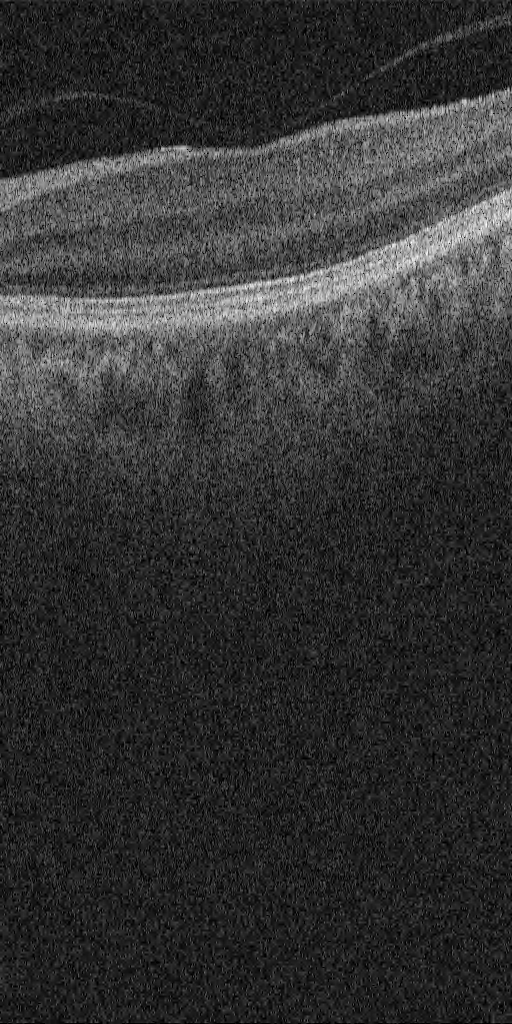
\includegraphics[scale=0.15]{normal_case.png}}\hfill
\subfigure[\ac{dme}-cyst]{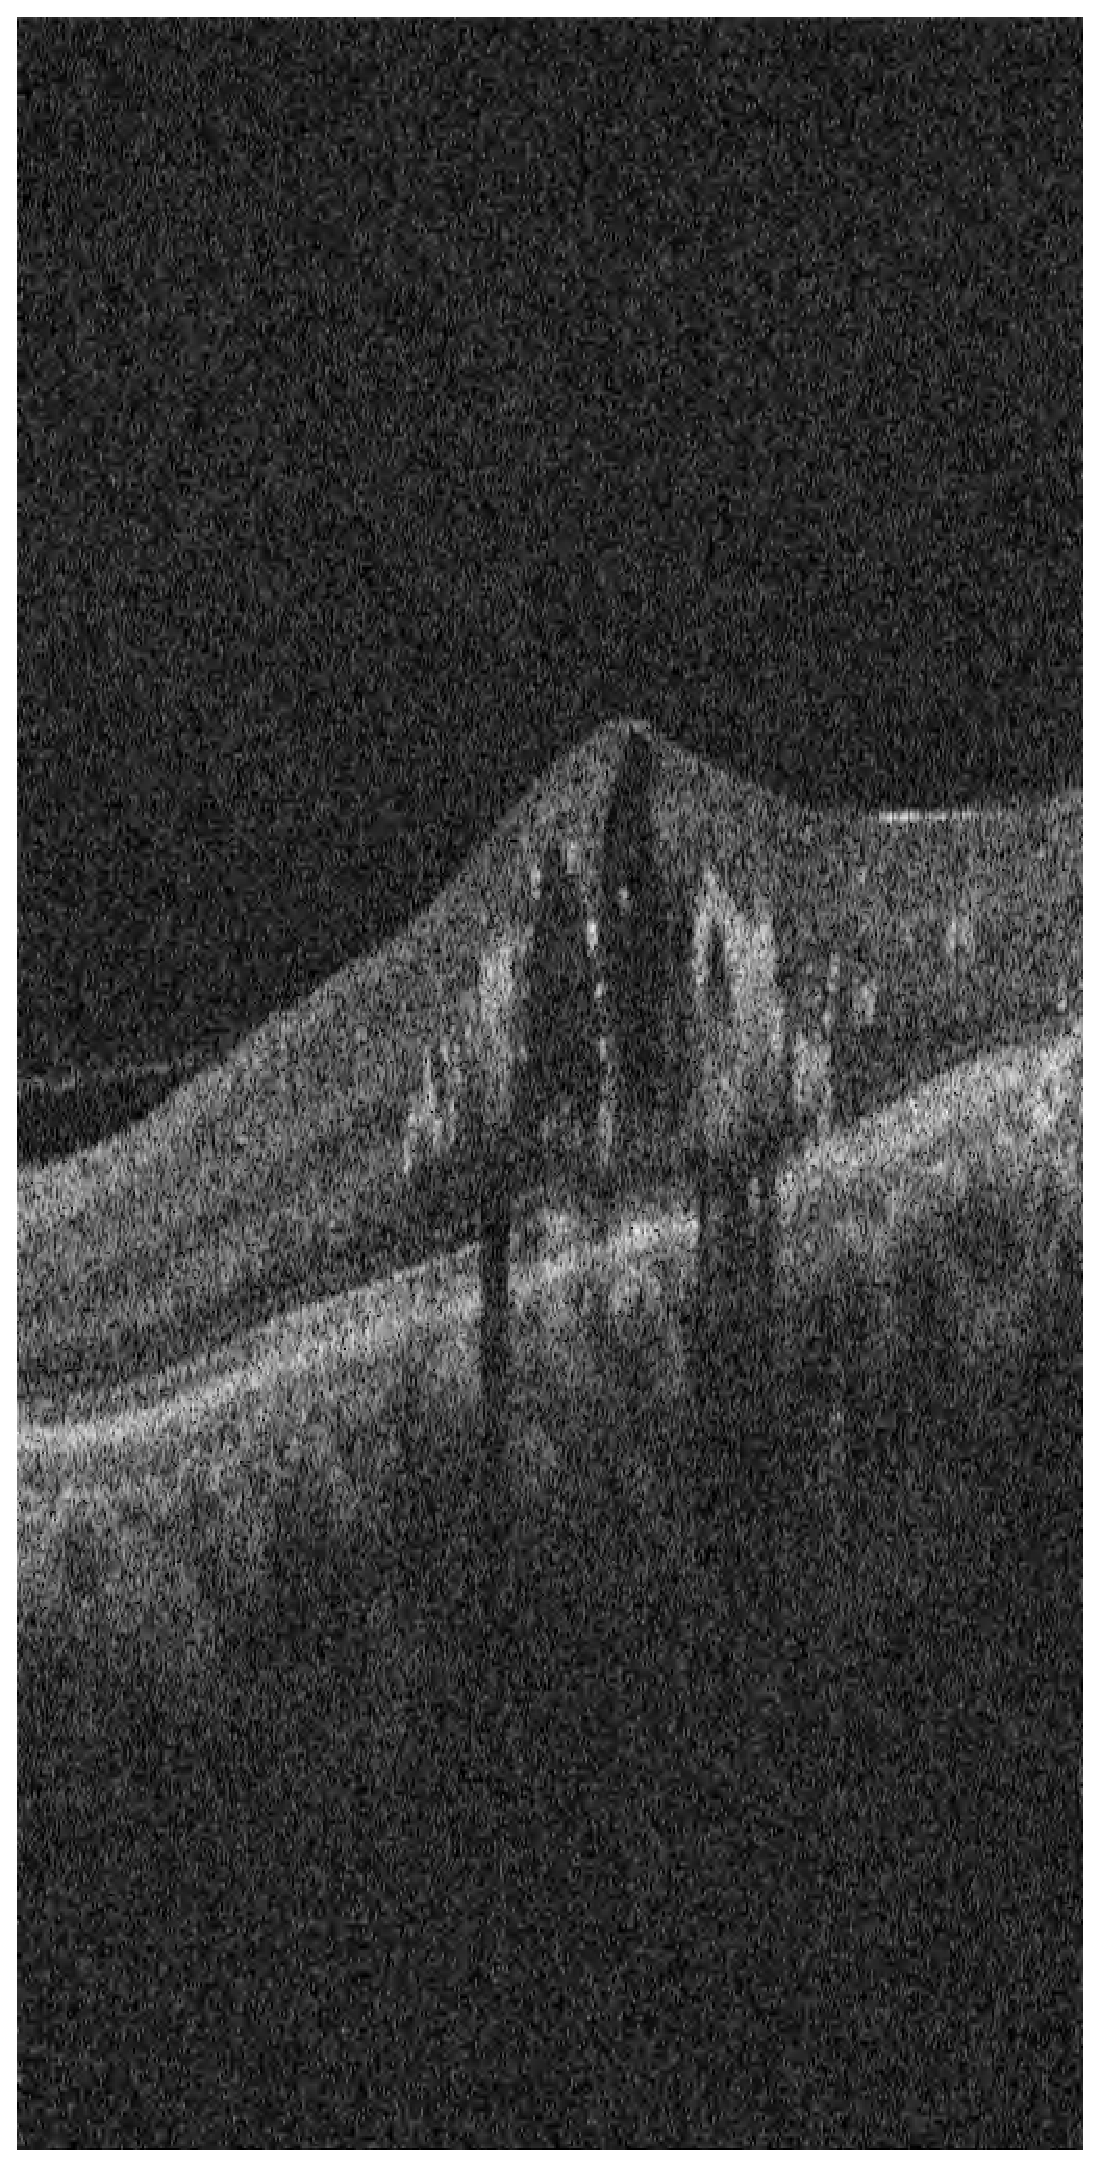
\includegraphics[scale=0.15]{dme_cyst}}\hfill
\subfigure[\ac{dme}-exudate]{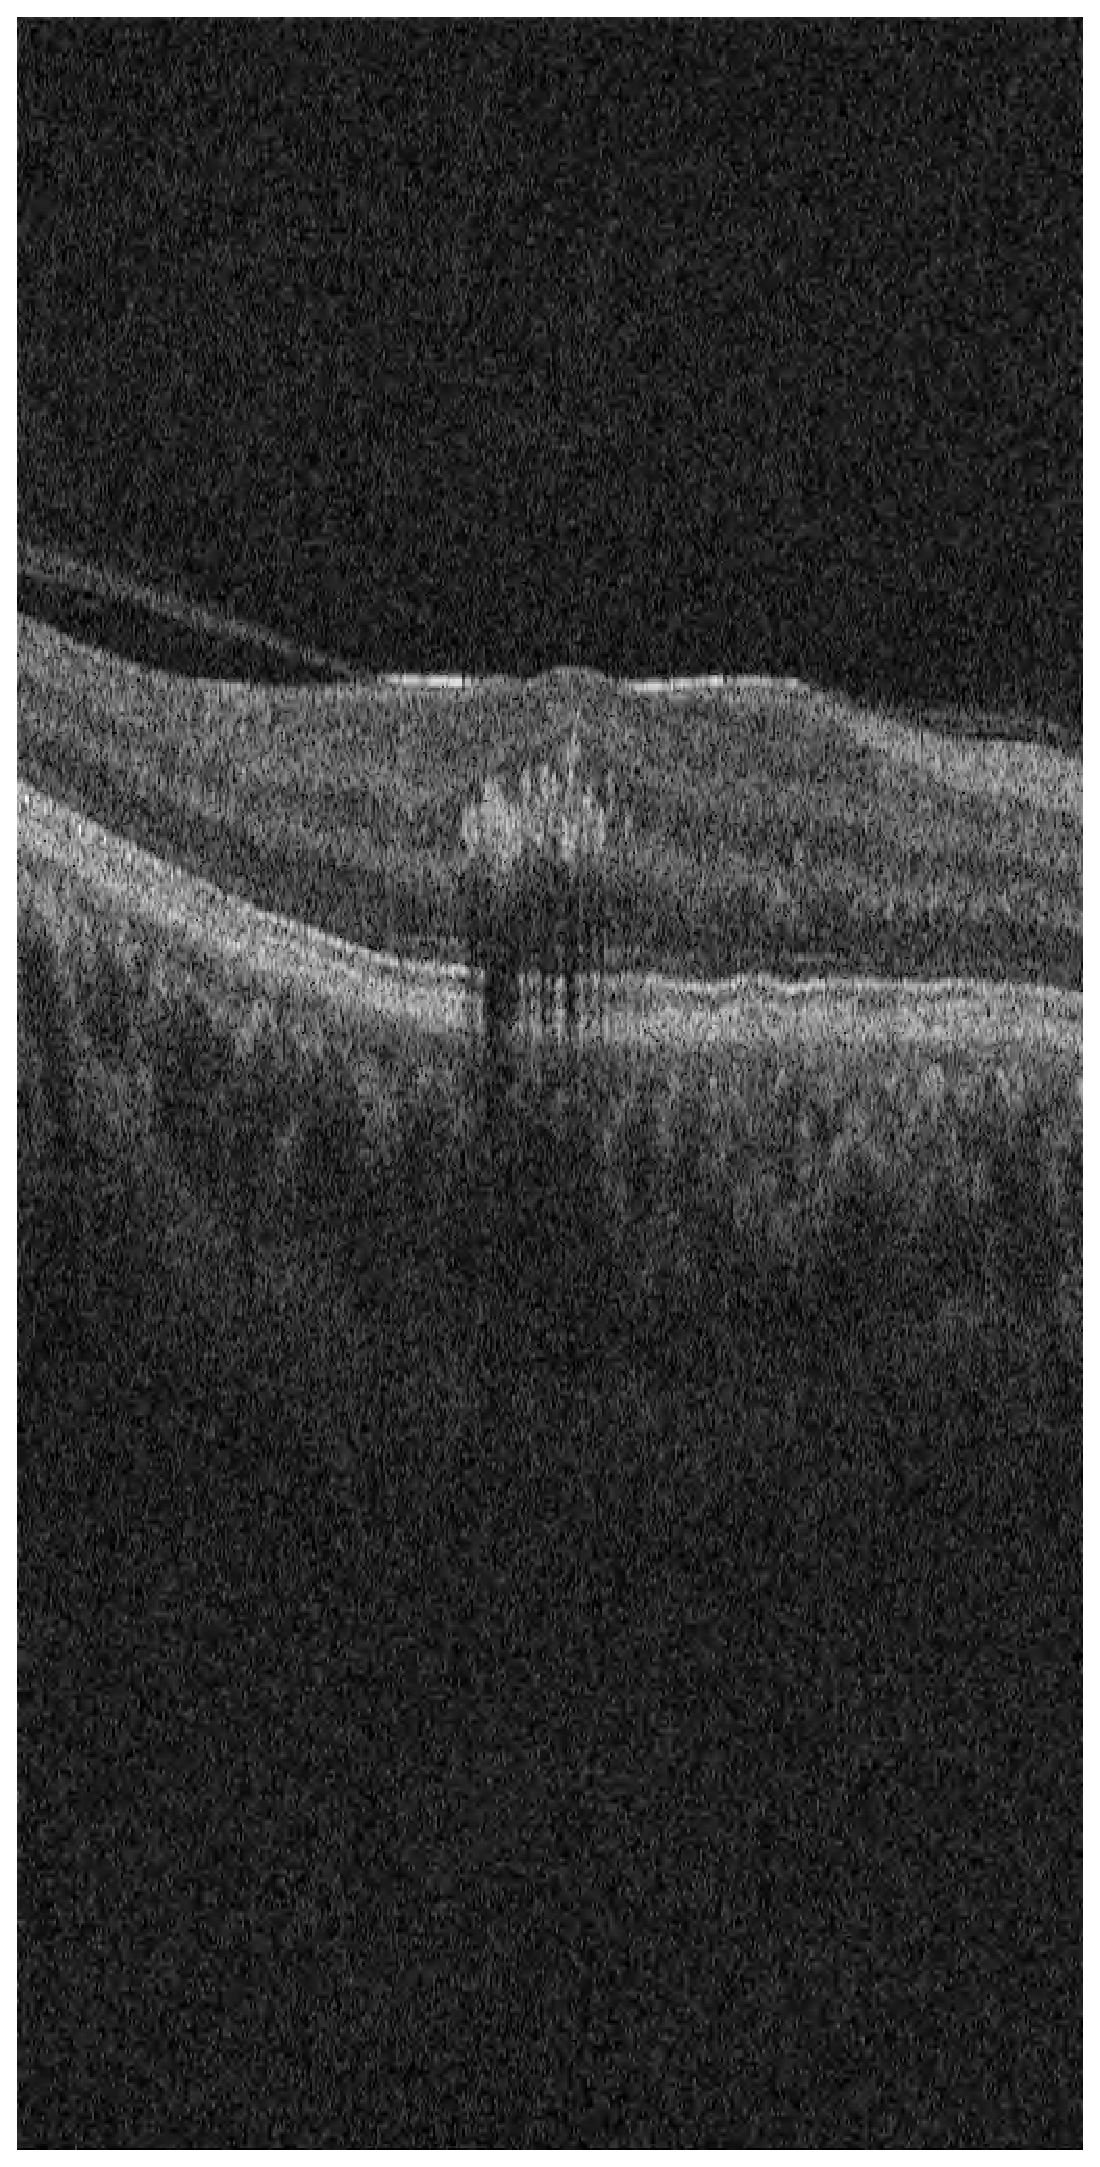
\includegraphics[scale=0.15]{dme_exudate}}
\hspace*{\fill}
\end{center}
\caption{ Example of \ac{sdoct} images for normal (a) and \ac{dme} patients (b)-(c) with cyst and exudate, respectively.}
\label{fig:dme-normal}
\end{figure}
\begin{changebar}
  \todo{I don't think thats the way to introduce it}
Many of the previous works on \ac{oct} image analysis have focused on the problem of retinal layers segmentation, which is a necessary step for retinal
thickness measurements~\cite{Chiu2010,Kafieh2013}.
However, few have addressed the specific problem of \ac{dme} and its associated features detection from \ac{oct} images.
\end{changebar}

In this research we focus on the latter problem and propose an automatic framework for identification of \ac{dme} patients versus normal subjects using \ac{oct} volumes.
The proposed method, which is an extension of our previous work \cite{Lemaintre2015miccaiOCT}, is based on \ac{lbp} features to describe the texture of \ac{oct} images and dictionary learning using the \ac{bow} models~\cite{Sivic2003}.
We propose to extract 2D and 3D \ac{lbp} features from \ac{oct} images and volumes, respectively.
The \ac{lbp} descriptors are further extracted from the entire sample or local patches within individual samples.
In this research beside the comparison of 2D and 3D features, we also compare the effects of common pre-processing steps for \ac{oct} data, study the optimal configuration regarding the \ac{bow} approach in conjunction with different base classifiers.

%In the following of this paper, first in Sect.\,\ref{sec:rw} a summary of the related studies is presented.

This paper is organized as follows, Section~\ref{sec:rw} presents a summary of the related studies.
The proposed framework is explained in Sect.\,\ref{sec:method}, while the experiments and results are discussed in Sect.\,\ref{sec:exp}.
Finally, the conclusion and avenue for future directions are drawn in Sect.\,\ref{sec:con}.


%----------

%%% Local Variables:
%%% TeX-master: "../../main.tex"
%%% TeX-master: "../../main.tex"
%%% End:
